\section{Introduction}\label{sec:intro}

Text-to-CAD systems turn natural-language descriptions into executable
parametric programs---typically CadQuery or construction-sequence code that is
rendered into boundary-representation (B-rep) geometry
\cite{deepcad,text2cad,llm4cad,cadrecode}. The promise is a conversational
interface to mechanical design; the reality is that users' descriptions are
almost always incomplete, occasionally self-contradictory, and rarely stated
at the level of precision a parametric program requires. Recent work addresses
this with \emph{proactive clarification}: an agent interrogates the prompt
before a second agent writes code \cite{procad}. ProCAD demonstrates that a
single round of questions, answered by an oracle user simulator, can recover
much of the geometry lost to underspecified or conflicting prompts.

Yet the two agents in this pipeline never share structured state. Their
\textbf{only hand-off is a single piece of free text}---a rewritten
``standardized prompt'' produced by the clarifier. Whatever the
question--answer exchange drops or invents is invisible to the coder;
whatever the coder ignores or improvises is invisible to everyone. There is
no execution-time feedback path either: generated code is evaluated only
offline, against ground-truth meshes that do not exist when the system is
deployed.

That this is not merely an aesthetic concern is suggested by two recent
findings from complementary angles. In verification-driven code generation,
vision--language models that inspect renders of their own CAD output can
catch some geometric errors iteratively \cite{cadcodeverify}---but their
validation questions and answers are both produced by the same model looking
at an image, with no grounded reference to what the user actually confirmed.
On the human side, Treellis \cite{treellis} shows that exposing the
\emph{structure} of a generated model lets users edit locally instead of
regenerating the whole object---yet only \textbf{32 of 50} generated models
were in an editable state on the first pass (43 after adding exemplars and
structural constraints). Exposing structure helps; the structure itself
remains ungrounded and unverified.

We argue that the missing object in this pipeline is a
\emph{provenance-tracked specification of design intent}, sitting between the
user and the coder: a structured feature graph in which every parameter
records \emph{where it came from}---stated by the user, confirmed in a
clarification answer, silently assumed by the system, or derived from a
constraint---and against which the generated program can be checked
\emph{without any ground-truth geometry}. Concretely, we introduce a
\textbf{Spec Manager} agent and a deterministic \textbf{spec-grounded
verifier}, and close the loop between them
(Figure~\ref{fig:overview}):

\begin{enumerate}
  \item \textbf{Structured, provenance-tagged specification
  (\S\ref{sec:spec}).} Instead of a rewritten prompt, the Spec Manager
  maintains a graph of features, parameters, and constraints. Clarification answers
  override earlier statements under an explicit provenance ranking; every
  override is logged in a machine-readable change record. Parameters the
  model fills in without user support are marked as assumptions rather than
  silently inserted. A deterministic kernel---not the LLM---owns merging,
  conflict resolution, and the detection of unresolved fields, so these
  invariants are unit-testable without an API call.

  \item \textbf{Ground-truth-free verification at deployment time
  (\S\ref{sec:verifier}).} The verifier aligns generated CadQuery code back
  to the \emph{specification the user confirmed}, not to a reference mesh. A
  static layer parses the program without executing it, maps its operations
  to specification fields, and flags confirmed values without a reliable
  mapping, dimensional literals with no source in the specification, and
  assumed values realized in code; a dynamic layer
  measures the executed B-rep directly (radii, depths, feature counts,
  topology) to catch the failure class numeric matching cannot---correct
  values with wrong operations, such as a hole that became a boss.

  \item \textbf{A closed loop with differential routing and a question
  budget (\S\ref{sec:loop}).} A missing \emph{assumption} is routed back to
  the user as a targeted question; a confirmed value the coder dropped is
  routed forward with a field-level diagnostic for grounded re-generation---
  the user is never re-asked what they already said. Triggered only on
  demand, the loop is designed to improve geometry under the same or smaller
  question budget than an unconditionally extra clarification round.
\end{enumerate}

We further show the behavior is reproducible without a proprietary model: the
Spec Manager distills into Qwen2.5-7B with training targets canonicalized by
the deterministic kernel, so the student cannot learn malformed schemas from
the teacher (\S\ref{sec:training}).

In a controlled re-creation of the ProCAD benchmark---underspecification and
direct-conflict prompts with severity $K{=}1..3$---we find that free-text
hand-offs lose or invent information in \RESULT{C1 rate} of clarified
samples, that such defects correlate with degraded Chamfer distance
(\RESULT{correlation}), and that the provenance specification reduces them to
\RESULT{C2 rate} while improving mean Chamfer distance from
\RESULT{E1 CD} to \RESULT{E3 CD} at \RESULT{rounds} average questions.
Crucially, verifier verdicts predict ground-truth geometric failure with
\RESULT{precision\slash recall}, establishing the deployment-time signal as a valid
proxy; and under imperfect (noisy or wrong) user answers---conditions the
oracle-simulator evaluation cannot examine---our pipeline degrades more
gracefully (\RESULT{C6 numbers}).

The central conceptual move is a separation the current literature conflates:
\emph{specification fidelity} (does the program realize what the user
confirmed?) from \emph{geometric similarity} (does the output resemble a
reference mesh?). Similarity needs ground truth and is available only in
evaluation; fidelity can be measured every time the system runs. Treellis
gives humans an editable geometric tree after generation; we give the agents a
grounded, traceable intent graph before generation and the means to check it
afterward---making an editable tree for people and a verified specification
for agents natural complements rather than competitors.

\begin{figure}[t]
  \centering
  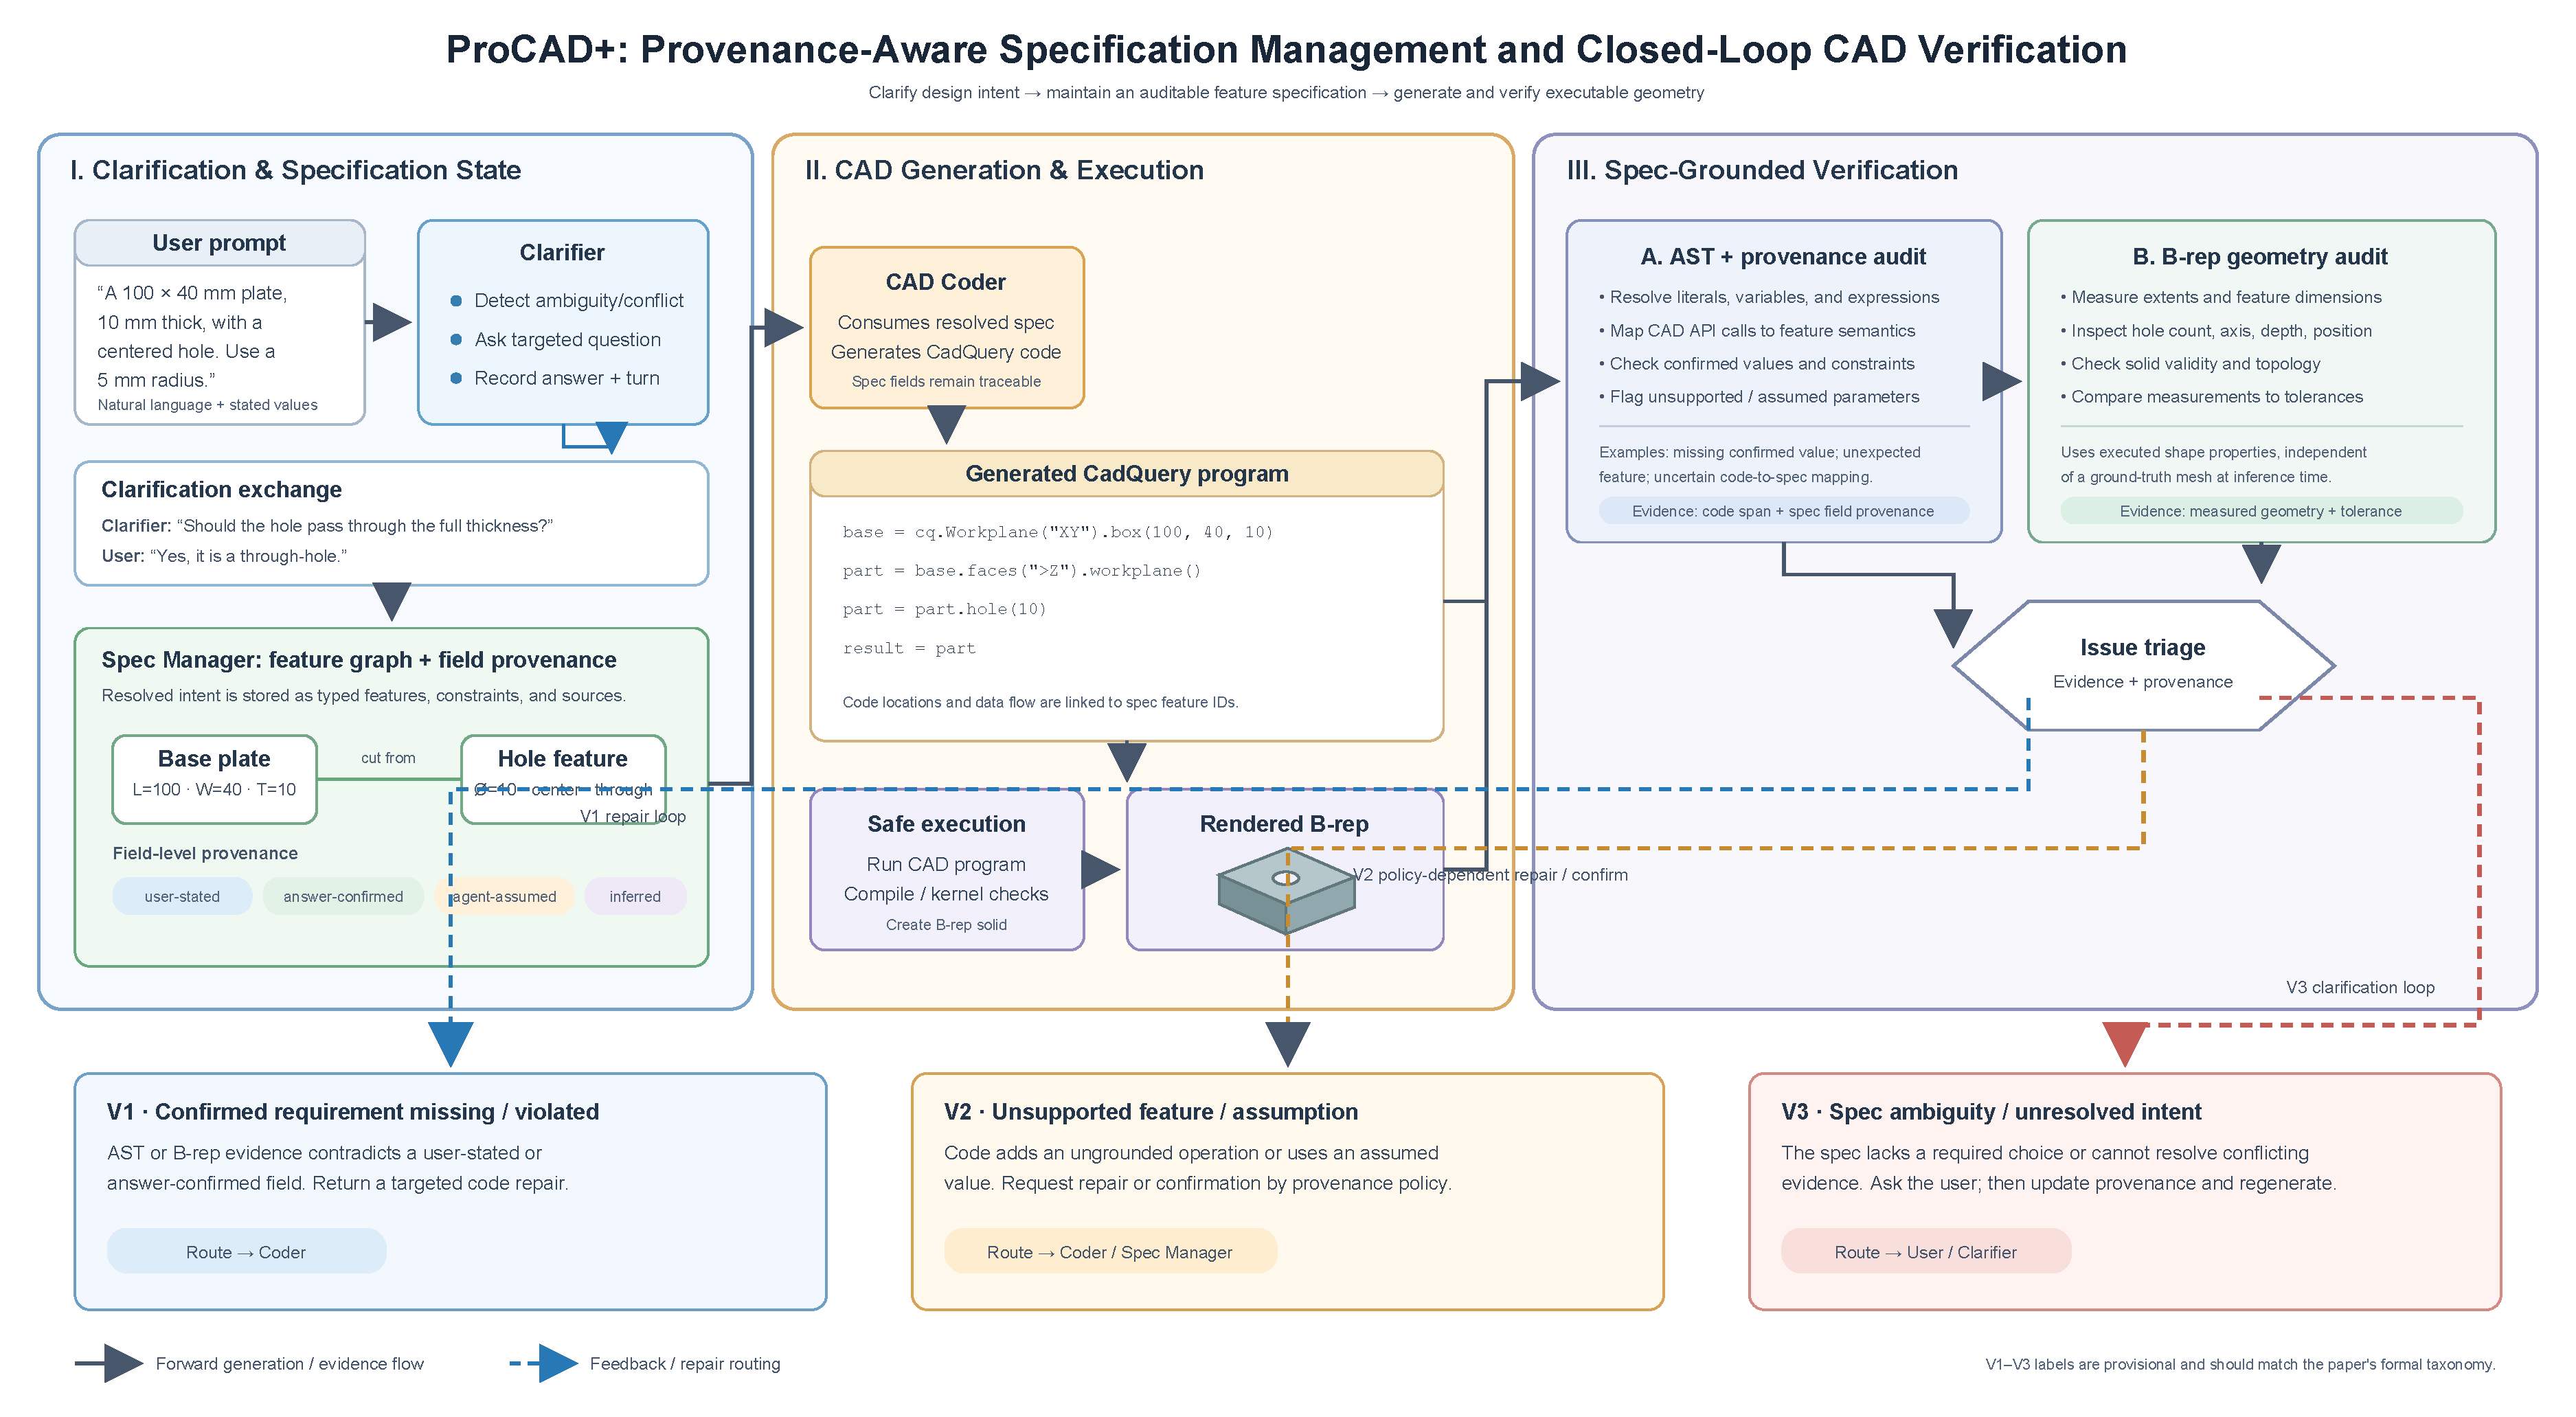
\includegraphics[width=\linewidth]{overview_figure.pdf}
  \caption{Pipeline overview. The specification is the single source of
  truth: it is grounded in the user's prompt and clarification answers,
  rendered for the coder, and used as the verification reference at
  deployment time, replacing the free-text hand-off and the ground-truth
  mesh.}
  \label{fig:overview}
\end{figure}
